Mit dieser Laborumgebung soll die Funktion einer Web Application Firewall (WAF) in drei Lerneinheiten vermittelt werden.
In dieser Lerneinheit sollen Sie sich mit der Lernumgebung vertraut machen und eine erste Konfiguration der WAF vornehmen.

\subsection{Vorbereitungen}
\label{sec:learning-unit-1-preparations}

Um die Laborumgebung zu nutzen werden die Folgenden Anwendungen benötigt:
\begin{itemize}
    \item \href{https://www.virtualbox.org/}{\underline{VirtualBox}}
    \item \href{https://code.visualstudio.com/download}{\underline{Visual Studio Code}}\\
    Die nicht quelloffene Version von Microsoft ist notwendig, da ein benötigtes Plugin in \textit{Open-Source} Distributionen wie \textit{vscodium} nicht verfügbar sind.
    \item Einen Web-Browser
\end{itemize}

\subsubsection{Virtuelle Maschine starten}
Importieren Sie nun die Virtuelle Maschine (VM),  die die Laborumgebung enthält in die VirtualBox Umgebung.
Die Datei (\textit{WAF-Laborumgebung.ova}) finden Sie im Moodle.

Bevor die VM gestartet werden kann, muss ein Host-Only Netzwerkadapter erstellt werden, um von ihrem Host-System auf die Services in der VM zugreifen zu können.
Die VM soll auf der IP-Adresse \textbf{192.168.56.2} aufrufbar sein.

Die folgende detaillierte Anleitung ist exemplarisch für Windows Systeme.
Wenn Sie ein anderes Betriebssystem oder eine andere Virtualisierungsumgebung nutzen, können Sie die Anleitung als Orientierung nutzen und müssen sich den Rest eigenständig erarbeiten.

\begin{enumerate}
    \item Den Netzwerk-Manager von VirtualBox aufrufen (\textit{File -> Tools -> Network Manager}).
    \begin{figure}[!hbt]
        \centering
        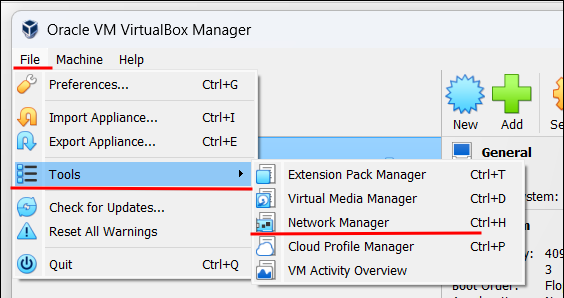
\includegraphics[width=0.5\textwidth]{./images/network-settings.png}
    \end{figure}
    \item Den Reiter \textit{Host-only Networks} auswählen.
    \item Mit \textit{Create} einen neuen Adapter erstellen.
    \item Die IPv4-Adresse muss auf 192.168.56.\textbf{1} konfiguriert sein damit die Virtuelle Maschine aufgefunden werden kann.
    \begin{figure}[!hbt]
        \centering
        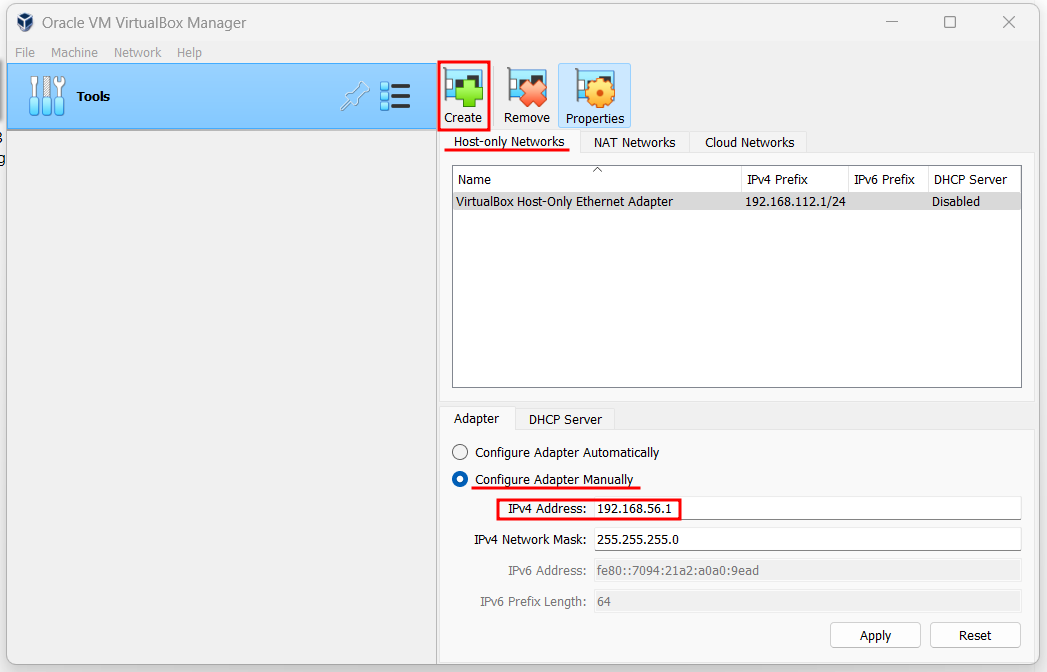
\includegraphics[width=0.9\textwidth]{./images/new-ho-network.png}
    \end{figure}
    \item Die Konfiguration der Laborumgebungs-VM aufrufen.
    \begin{figure}[!hbt]
        \centering
        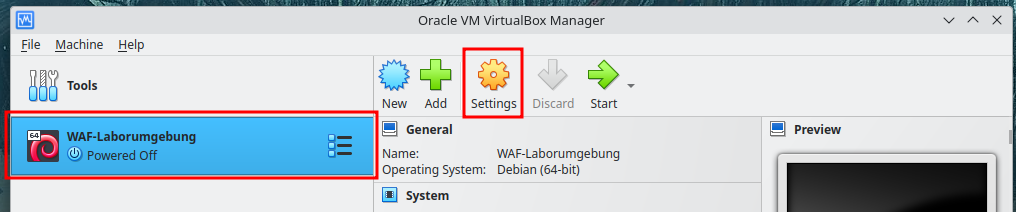
\includegraphics[width=0.9\textwidth]{./images/vm-settings.png}
    \end{figure}
    \item Den zweiten Netzwerk-Adapter unter (\textit{Network -> Adapter 2}) aktivieren.
    \item Den in Schritt 3 erstellten Adapter der VM zuordnen
    \begin{figure}[!hbt]
        \centering
        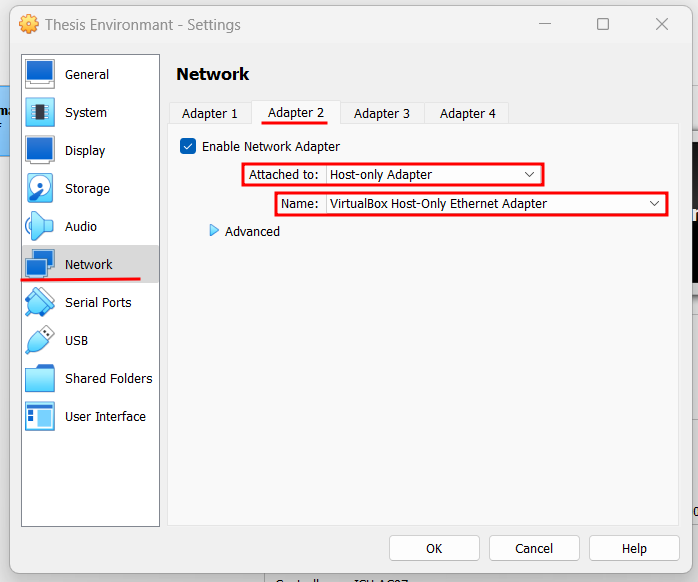
\includegraphics[width=0.9\textwidth]{./images/vm-ho-config.png}
    \end{figure}
\end{enumerate}
\pagebreak

Jetzt kann die Virtuelle Maschine gestartet werden.

\subsubsection{Websites aufrufen}
Die Lernumgebung bietet mehrerer Services mit denen interagiert werden kann, die alle mit Hilfe der Containervirtualisierungsumgebung Docker verwaltet werden.
Unter \href{https://192.168.56.2:9443}{\underline{https://192.168.56.2:9443}} steht eine Docker-Weboberfläche zur Verfügung, um die Bedienung zu erleichtern.
Die Login Daten sind:
\begin{itemize}
    \item \textbf{Username:} admin
    \item \textbf{Passwort:} waf-env12345
\end{itemize}

Nach einem Neustart der VM muss der WAF Docker-Container neu gestartet werden.
Auch wenn die WAF-Konfiguration geändert wurde, muss die WAF neugestartet werden damit die Änderungen übernomen werden.

Nach dem Login muss als erstes das lokale Environment und der Docker-Stack ausgewählt werden.
Dann kann die Laborumgebung (neu) gestartet werden:
\pagebreak

\begin{enumerate}
    \item \textit{Stacks -> waf-enf} auswählen
    \begin{figure}[!hbt]
        \centering
        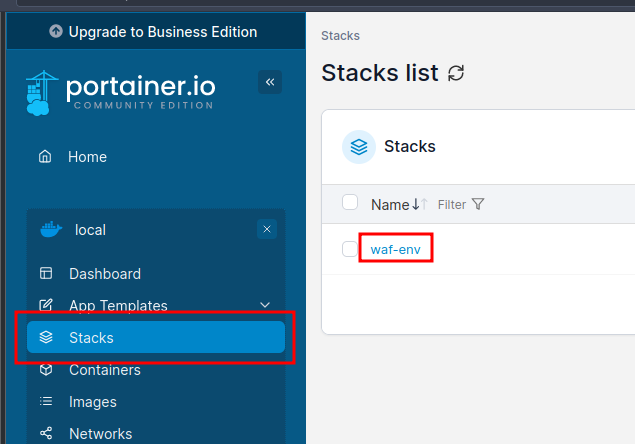
\includegraphics[width=0.9\textwidth]{./images/waf-env-porteiner.png}
    \end{figure}
    \item Hier können die Container ausgewählt und neugestartet werden
    \begin{figure}[!hbt]
        \centering
        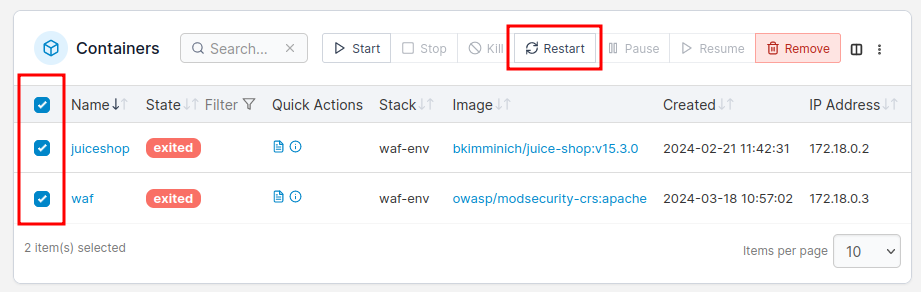
\includegraphics[width=\textwidth]{./images/restart-all.png}
    \end{figure}
\end{enumerate}

Nun sind alle Services der Laborumgebung aktiv und sind unter den folgenden URLs abrufbar:
\begin{enumerate}
    \item Verwundbare Anwendung mit WAF \href{https://192.168.56.2:443}{\underline{https://192.168.56.2:443}}
    \item Verwundbare Anwendung ohne WAF \href{http://192.168.56.2:3000}{\underline{http://192.168.56.2:3000}}
    \item Portainer \href{https://192.168.56.2:9443}{\underline{https://192.168.56.2:9443}}
\end{enumerate}

\subsubsection{Die WAF Konfigurationsdatei bearbeiten}

Der letzte Schritt zur Vorbereitung der Umgebung ist der Zugriff auf die WAF-Konfiguration.
Dies erfolgt über SSH auf die Virtuelle Maschine.
In dieser Anleitung wird die Verbindung mit der \textit{Visual Studio Code} Extension \href{https://marketplace.visualstudio.com/items?itemName=ms-vscode-remote.remote-ssh}{\underline{Remote - SSH}} erläutert.
Der Zugriff ist jedoch auch mit jedem anderen SSH-Client möglich.

\begin{itemize}
    \item \textbf{URL:} 192.168.56.2:22
    \item \textbf{Username:} waf-env
    \item \textbf{Passwort:} waf-env
\end{itemize}

Ist die Extension in vscode installiert, kann unter \textit{Remote Explorer -> SSH} mit dem \textit{+}-Icon eine neue Verbindung angelegt werden.

\begin{figure}[!hbt]
    \centering
    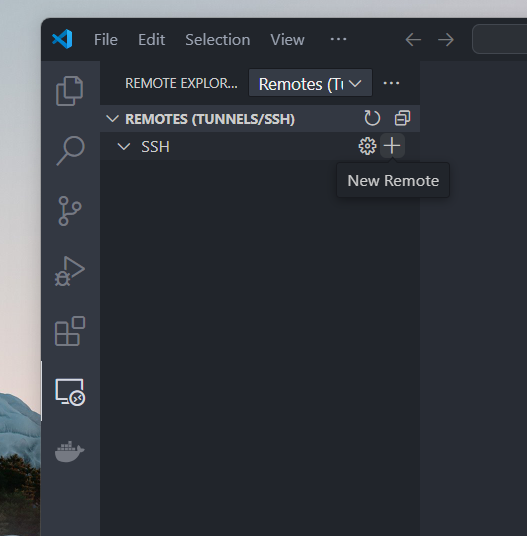
\includegraphics[width=0.5\textwidth]{./images/vscode-new-ssh.png}
\end{figure}

In dem sich öffnenden PopUp muss die SSH Verbindung eingetragen werden:

\textbf{waf-env@192.168.56.2}.

\begin{figure}[!hbt]
    \centering
    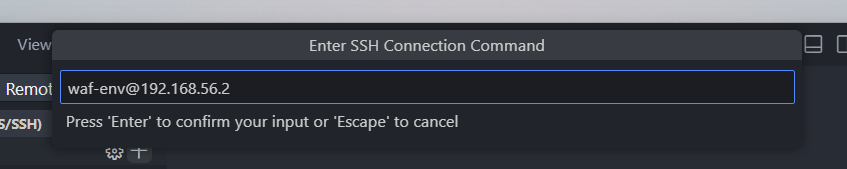
\includegraphics[width=0.9\textwidth]{./images/vscode-ssh-string.png}
\end{figure}

Es folgen PopUps in denen nach dem Gast Betriebssystem (Linux) und der Konfigurationsdatei für ssh gefragt werden.
Nutzen Sie die vorgeschlagenen Optionen.

Während dem Prozess wird wiederholt nach dem Passwort (\textit{waf-env}) gefragt.

Ist die Konfiguration abgeschlossen kann die Verbindung zu der VM mittels des Popups in der rechten unteren Ecke aufgebaut werden.

\begin{figure}[!hbt]
    \centering
    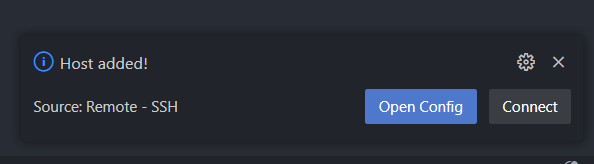
\includegraphics[width=0.7\textwidth]{./images/vscode-connect.png}
\end{figure}

Nachdem die Verbindung aufgebaut wurde muss zu dem Ordner navigiert werden, der die Konfigurationsdateien und Logs der WAF enthalten.

Im Reiter \textit{Explorer} kann der Ordner geöffnet werden.

\begin{figure}[!hbt]
    \centering
    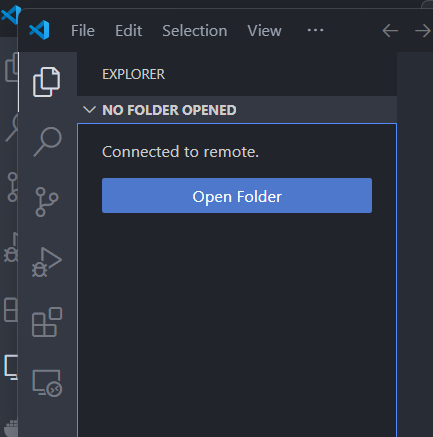
\includegraphics[width=0.7\textwidth]{./images/vscode-initiate-nw-dir.png}
\end{figure}

In dem PopUp den Pfad \textit{/home/waf-env/waf-env} angeben und bestätigen.

\begin{figure}[!hbt]
    \centering
    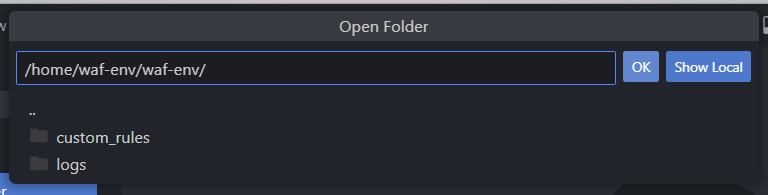
\includegraphics[width=0.7\textwidth]{./images/vscode-dir-path.png}
\end{figure}

Visual Studio Code merkt sich die Konfiguration die bei wiederholtem Aufruf im \textit{Remote Explorer} aufgerufen werden kann.

\subsection{Erste Konfiguration}

Die Ressourcen die Sie in der folgenden Liste finden, können Ihnen bei der Bearbeitung der Aufgabenstellungen behilflich sein.

\begin{itemize}
    \item Das \href{https://github.com/owasp-modsecurity/ModSecurity/wiki/Reference-Manual-(v3.x)}{\underline{ModSecurity Refernece Manual}} besonders die  \href{https://coreruleset.org/docs/rules/creating/}{\underline{Anleitung zum Schreiben von Regeln}}
    \item Auflistung der \href{https://pwning.owasp-juice.shop/companion-guide/latest/part2/README.html}{\underline{OWASP Juice Shop Challenges}}
    \item \href{https://github.com/refabr1k/owasp-juiceshop-solutions/tree/master}{\underline{Beispiellösungen}} für den Juice Shop
    \item Der Progress tracker des Juice Shops der unter der URL \textit{/\#/score-board} zu finden ist
\end{itemize}

\subsubsection{Sperren eines Pfades}
Um sich mit dem Aufbau einer ModSecurity Regel vertraut zu machen, soll der Zugang zu einem Pfad in der Website gesperrt werden.

In der Challenge \glqq\href{https://pwning.owasp-juice.shop/companion-guide/latest/part2/sensitive-data-exposure.html#_access_a_confidential_document}{\underline{access a confidential document}}\grqq\ ist der Zugriff auf ein Dokument möglich.

\textbf{Schreiben Sie eine neue Regel, die den Zugriff auf dieses Dokument verhindert und mit dem HTTP-Fehlercode 401 antwortet.}

\subsubsection{Parsen von HTTP Parameter}
In der Challenge \glqq\href{https://pwning.owasp-juice.shop/companion-guide/latest/part2/improper-input-validation.html#_give_a_devastating_zero_star_feedback_to_the_store}{\underline{give a devastating zero-star feedback to the store}}\grqq\ kann durch Bearbeiten eines HTTP-Requests ein Produkt mit 0 Sternen bewertet werden.

Vollziehen Sie das beschriebene Problem nach:
\begin{itemize}
    \item Was ist der Fehler, der die Schwachstelle ermöglicht?
    \item Welcher Parameter enthält die schadhaften Daten?
    \item Was wäre das korrekte Verhalten?
\end{itemize}

\textbf{Wenn Sie die Schwachstelle verstanden haben, schreiben Sie eine weitere Regel, die verhindert, dass ein Angreifer keine Daten außer den gültigen Werten an den Endpoint senden kann.}

\pagebreak